\chapter{Implementare, teste}

În aceast capitol vom prezenta aplicația, începând de la arhitectură, continuând apoi spre funcționalitatea oferită. Idea este să punem in aplicare conceptele teoretice de la capitolele anterioare, punând accent pe algoritmii de la secțiunea Aritmetica Eficienta, capitolul 2. Implementarea eficientă si corectă a acestor operații reprezintă un prim pas foarte important spre dezvoltarea de aplicații criptografice folosite în lumea reală, precum ECDSA.
\\ Pentru implementare am ales limbajul de programare Python, versiunea 3.5.2, iar hardware-ul folosit in tabelele de test este: Quad Core CPU, i7-4700HQ, 2.4 GHz, 64 bit OS, 16 GB RAM.

\section{Arhitectura Aplicației}
%arhitectura(Inclusiv grupul folosit, curbele eliptice Nist), diagrama UML cu clasele
În această aplicație s-a urmărit scrierea unui cod cât mai flexibil și concis, care să permită manipularea și aprofundarea conceptelor abstracte, matematice, discutate în secțiunile predente. Scopul final al aplicației a fost implementarea protocolul \textit{ECDSA} și un studiu comparativ al performanței algoritmilor discutati in Capitolul 2, Secțiunea Aritmetică Eficientă. \\
Deși limbajul folosit suportă atât paradigma de programare orientată pe obiecte, cât si cea procedurală, în această aplicație am ales structurarea aproape completă a codului în clase, fiecare cu roluri bine definite, pe cât posibil în concordanță cu principiile \textit{SOLID}\cite{solid}, fară însă a face compromisuri în ceea ce privește flexibilitatea si simplitatea codului. Diagrama \textit{UML}\cite{uml} din figura 4.1 surprinde toate clasele din aplicație si relațiile dintre acestea. Se observă folosirea unor clase abstracte, deși nu există suport nativ pentru ele în Python. Acestea au fost folosite pentru a reduce multe din reduntanțele care apăreau în cod și pentru a oferi un sablon pentru anumite funcționalități care pot fi introduse în aplicație. Abstractizarea claselor în Python se face cu ajutorul pachetului \textit{abcMeta}\cite{abcMeta}.\\
Funcționalitatea oferită de protocolul ECDSA, adică generarea cheilor, semnarea mesajului si verificarea semnăturii este încapsulată în 3 clase: \textit{GenerateKeyPair}, \textit{GenerateSignature}, \textit{VerifySignature}. Algoritmii care vor apărea în Studiul Comparativ sunt implementați în clasele \textit{ScalarMultiplication} și \textit{JointMultiplication}. În continuare, voi prezenta structurile de date care stau la baza aplicației.

\begin{figure}[htp]
\centering
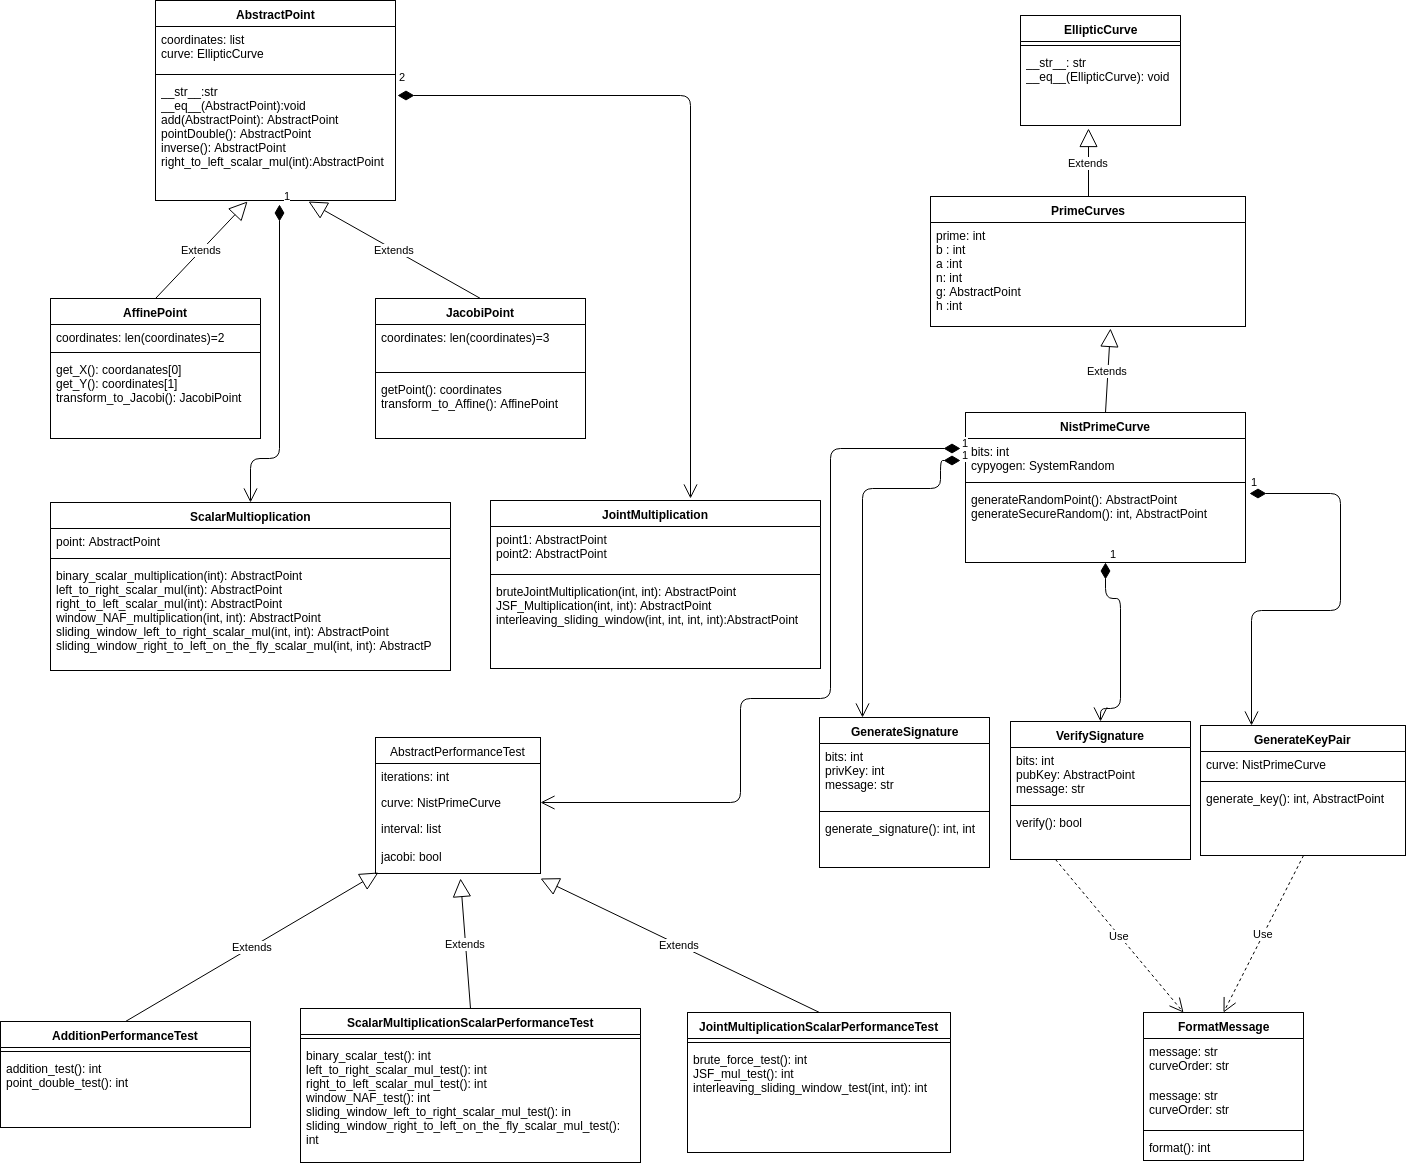
\includegraphics[width=17.5cm]{chapters/Arhitectura.png}
\caption{Arhitectura Aplicației}
\label{fig:lion}
\end{figure}

\subsection{Structuri de date}

În aplicație a fost necesară modelarea a două entități fundamentale, curba eliptică și punctul de pe o curbă eliptică. Pentru ambele concepte am creat clase abstracte, întrucât există multe tipuri de curbe eliptice, iar punctele pot avea și ele mai multe reprezentări.

\subsubsection{Curba Eliptică}
Am ales sa modelez conceptele de curbă eliptică peste un corp prim(clasa concretă \textit{PrimeCurves}) și extensia acesteia care modelează curbele NIST peste corpuri prime, \textit{NistPrimeCurve}. Clasa abstractă pentru o curbă eliptică este special modelată vag, din cauza multitudinii de tipuri de curbe existente, cu proprietăți specifice foarte speciale. Clasa \textit{PrimeCurves} modelează orice curbă definită peste un corp prim si în afara parametrilor care definesc curba si a supraîncărcării operatorilor de egalitate si de reprezentare string a obiectului, am decis să nu adaug metode speciale. Curbele Nist, definite peste corpuri prime si modelate în clasa \textit{NistPrimeCurve} au parametrii cunoscuți, definiți în \cite{nist}.

\subsubsection{Punctele de pe o curbă eliptică}

Am modelat punctele reprezentate in coordonate afine (\textit{AffinePoint}) și punctele în coordonate jacobiene (\textit{JacobiPoint}).
Design-ul punctelor a fost conceput în așa fel încat fiecare punct să conțină metode pentru operațiile de grup pentru curbe eliptice: adunare, dublare, invers. De asemenea, fiecare punct, are coordonate si aparține unei curbe, lucru reflectat în constructorul clasei \textit{AbstractPoint}. Am luat decizia să nu adaug in clasele pentru puncte metode de înmulțire cu un scalar sau de înmulțire multiplă deoarece cei mai eficienți algoritmi necesită precalcularea unor valori, acest lucru adaugând un overhead clasei punct. Astfel, cel mai eficient algoritm de înmultire a fost separat într-o clasă, care se ocupă special de această operație La fel am procedat și cu operația de înmulțire multiplă. \\

Abstractizarea acestor concepte ajută la eventuala extindere a aplicației și la evitarea codului duplicat. Prin extinderea claselor abstracte, putem adauga suport pentru alte tipuri de curbe eliptice, precum cele definite peste corpuri binare, curbe Edwards, sau suport pentru diferite tipuri de coordonate și operațiile speciale aferente.


\section{Aritmetică}
\label{subsec:subsec02}
În această secțiune vom aborda operațiile de grup pentru curbe eliptice, adunare, dublare, invers și operațiile speciale, înmulțirea cu un scalar și înmulțirea multiplă. Cele din urmă au fost explicate în capitolul doi, secțiunea Aritmetică Eficientă. Aici ne vom concentra pe implementarea acestora și rolul acestora în Studiul Comparativ, respectiv în protocolul ECDSA. \\

Justifici clasele ScalarMultiplier, zici ca prezinti  atat aritmetica de grup cat si cea speciala... 

\subsection{Operații de Grup}
În aplicatie am implementat operațiile care țin de grupul punctelor de pe o curbă eliptică în cele doua clase concrete pentru puncte, cele pentru coordonate afine si pentru coordonate jacobiene. Algoritmii de adunare constau în aplicarea unor formule, cele pentru coordonate afine fiind explicitate în Capitolul 2, Secțiunea Grupul Punctelor de pe o curba eliptică. Formulele de adunare și dublare a unui punct pentru coordonate Jacobiene sunt conform acestei surse \cite{jacobian}.

Operațiile care țin de structura de grup au o importanță deosebită, întrucât sunt folosite în fiecare algoritm de înmulțire cu scalar și implicit de înmulțire multiplă. Din acest motiv, ne dorim o implementare cât mai eficientă, orice înbunătățire la acest nivel aducând sporuri de performanță peste tot în aplicație. În coordonate afine, apare algoritmul lui Euclid Extins în calculul unor inverși modulari, astfel justificând folosirea coordonatelor jacobiene, care prin introducerea unui set de redundanțe în reprezentarea unui punct, elimină nevoia de a calcula inverși modulari. În continuare vom prezenta implementarea adunării și dublării unui punct în coordonate jacobiene. 

\begin{lstlisting}[language=Python]
def add(self, other):
    if self is None:
        return other
    if other is None:
        return self

    u1 = (self.x * other.z ** 2) % self.curve.prime
    u2 = (other.x * self.z ** 2) % self.curve.prime
    s1 = (self.y * other.z ** 3) % self.curve.prime
    s2 = (other.y * self.z ** 3) % self.curve.prime
    if u1 == u2:
        if s1 != s2:
            return None
        else:
            return self.point_double()

    h = (u2 - u1) % self.curve.prime
    r = (s2 - s1) % self.curve.prime
    x3 = (r ** 2 - h ** 3 - 2 * u1 * h ** 2) % self.curve.prime
    y3 = (r * (u1 * h ** 2 - x3) - s1 * h ** 3) % self.curve.prime
    z3 = (h * self.z * other.z) % self.curve.prime
    return Jacobi_Point([x3, y3, z3, pow(z3, 2, self.curve.prime), 
           pow(z3, 3, self.curve.prime)], self.curve)
\end{lstlisting}

\begin{lstlisting}[language=Python]
def point_double(self):
    if self is None:
        return None
    if self.y == 0:
        return None
    s = (4 * self.x * self.y ** 2) % self.curve.prime
    m = (3 * self.x ** 2 + self.curve.a * self.z ** 4) % self.curve.prime
    _x = (m ** 2 - 2 * s) % self.curve.prime
    _y = (m * (s - _x) - 8 * self.y ** 4) % self.curve.prime
    _z = (2 * self.y * self.z) % self.curve.prime
    return Jacobi_Point([_x, _y, _z, pow(_z, 2, self.curve.prime), 
	   pow(_z, 3, self.curve.prime)], self.curve)
\end{lstlisting}

Atât în coordonate afine, cât și în cele jacobiene, inversul unui punct este foarte simplu de calculat, prin negarea componentei a doua din reprezentarea punctului. Singurul dezavantaj al folosirii coordonatelor jacobiene îl constituie operația de trecere înapoi în coordonate afine, operație care necesită calcului a doi inverși modulari.

\begin{lstlisting}
def transform_to_affine(self):[language=Python]
       return AffinePoint([self.coordinates[0] * inv(self.coordinates[2] ** 2, 	    self.curve.prime) % self.curve.prime, (self.coordinates[1] * inv(self.coordinates[2] ** 3  3, self.curve.prime)) % self.curve.prime], self.curve)
\end{lstlisting}

\subsection{Înmulțirea cu un scalar}

Putem aborda problema înmulțirii cu un scalar în diferite feluri, de la cele mai ineficiente metode(apelararea functiei de adunare de cate ori este nevoie) până la metode sofisticate și eficiente, cum ar fi înmulțirea cu fereastră glisantă.

Cel mai eficient algoritm, rezultat în urma Studiului Comparativ, a fost încapsulat în clasa \textit{FastScalarMultiplier}. 

\subsubsection{Metoda Binară}

Prima metodă pe care am implementat-o este cea binară. Algoritmul constă în procesarea reprezentării binare a scalarului de la cel mai nesimnificativ bit la cel mai semnificativ.

\begin{lstlisting}[language=Python]
def binary_scalar_multiplication(self, d):
    P = self.point
    if d == 0:
        return None
    if d == 1:
        return P
    result = None
    while d > 0:
        if d % 2:
            result = P.add(result)
        d //= 2
        P = P.add(P)
    return result
\end{lstlisting}

În variabila \textit{result}, ținem rezultatul după fiecare iterație, iar în variabila $P$ ținem o copie punctului care dorim să îl înmulțim. Astfel, după fiecare bit parcurs dublăm $P$ și când întâlnim un bit de $1$ adunăm la rezultat $P$. La final returnăm variabila \textit{result}.

\subsubsection{Reprezentări cu semn}

Un avantaj major al grupului punctelor de pe o curbă eliptică îl reprezintă calculul foarte ușor din punct de vedere computațional al inversului. Astfel, putem să apelăm la reprezentările cu semn pentru scalar, acestea optimizând calculul de înmulțire cu un scalar. Cea mai eficientă astfel de reprezentare este $NAF$. \\

În continuare voi prezenta un algoritm pentru calculul reprezentării $NAF$. \\

\begin{lstlisting}[language=Python]
def naf(d):
    i = 0
    res = []
    while d >= 1:
        if d % 2 == 0:
            res.append(0)
        else:
            res.append(2 - d % 4)
            d -= res[i]
        d //= 2
        i += 1
    return res[::-1]
\end{lstlisting}

Cifrele care formează reprezentarea  $NAF$ sunt generate de resturile împărțirii repetate a scalarului la $2$. Această împărțire este una cu semn, resturile putând fii $\set{0, 1, -1}$. Când, în bucla \textit{while}, scalarul $d$ este impar și trebuie sa alegem între $r\in\set{-1, 1}$, alegem în așa fel încât $\frac{d-r}{2}$ să fie par, astfel făcând ca următoarea cifră din $NAF$ să fie $0$.

Având la dispoziție metoda pentru aflarea reprezentării cu semn a unui numar natural, putem eficientiza metoda binară. Algoritmul de la stânga la dreapta pentru calculul lui $dP$, unde d este scalarul si $P$ este un punct de pe o curba eliptica, apelează funcția pentru reprezentare cu semn. Parcurgem aceasta, dublând cantitatea din variabila \textit{result} după fiecare bit parcurs, iar la bitul de 1 adunăm punctul $P$, la bitul $-1$ scadem $P$ din rezultat. Urmează implementarea acestui algoritm.

\begin{lstlisting}[language=Python]
def left_to_right_scalar_mul(self, d):
    signed_d = naf(d)
    result = None
    for i in signed_d:
        if result is None:
            result = None
        else:
            result = result.point_double()
        if i == 1:
            result = self.point.add(result)
        if i == -1:
            result = self.point.inverse().add(result)
    return result
\end{lstlisting}

Algoritmul de la dreapta la stânga funcționează în același mod, singura diferență fiind faptul că NAF-ul este calculat în aceași buclă while în care calculăm rezultatul final. În acea buclă descompunem scalarul, ținem bit-ul curent într-o variabilă, $u$, iar apoi în funcție de valoarea acestuia modificăm rezultatul. Cei doi algoritmi au aceași complexitate asimtotică.

\begin{lstlisting}[language=Python]
def right_to_left_scalar_mul(self, d):
    result = None
    R = self.point
    while d >= 1:
        if d % 2 == 1:
            u = 2 - (d % 4)
            d -= u
            if u == 1:
                result = R.add(result)
            else:
                result = R.inverse().add(result)
        d //= 2
        R = R.point_double()
    return result
\end{lstlisting}

\subsubsection{Metoda cu fereastră}

Metoda cu fereastră poate fi privită ca o generalizare a metodei cu semn, aceasta aducând plusuri de performanță în schimbul folosirii unui plus de memorie. Această metodă se folosește de reprezentarea $w-NAF$ a scalarului.
Un algoritm eficient pentru calculul $w-NAF$ va fi prezentat în continuare. Funcția mods este modulo cu semn, adica pentru un scalar $d$, avem $d$ mods $2^w=u$, unde u este un numar intreg care satisface $u\equiv d$ mod $2^w$ si $-2^{w-1}\leq u\leq 2^{w-1}$.

\begin{lstlisting}[language=Python]
def w_NAF(d, w):
    i = 0
    res = []
    while d >= 1:
        if d % 2 == 0:
            res.append(0)
        else:
            res.append(mods(d, w))
            d -= res[i]
        d //= 2
        i += 1
    return res[::-1]
\end{lstlisting}

Se observă că cifrele din $w-NAF$ sunt de fapt restul împărțirii cu semn a scalarului la $2$, rest care aparține intervalului $[-2^{w-1}, 2^{w-1}-1]$. Astfel, daca scalarul $d$ este impar și $r = d$ mods $2^w$, atunci $\frac{d-r}{2}$ este divizibil cu $2^{w-1}$, asigurând astfel ca următoarele $w-1$ cifre din reprezentare sunt $0$.
 
Metoda cu fereastră aduce un plus de performanță prin reducerea numărului de adunări necesare în calculul multiplului unui punct oarecare $P$ de pe o curbă eliptică. Aici vom folosi reprezentarea $w-NAF$ in loc de $NAF$. Vom precalcula și stoca valorile pentru $iP$ si $i\in\set{1, 2^{w-1}}$. Astfel, când parcurgem $w-NAF$ -ul numarului, în funcție de cifra gasită vom aduna sau scădea din rezultat valorile potrivite din multimea de valori precalculate, dublând variabila acumulator la fiecare iterație.

\begin{lstlisting}[language=Python]
def window_NAF_multiplication(self, d, w):
    d = w_NAF(d, w)
    Q = None
    for i in range(0, len(d)):
        if Q is None:
            Q = None
        else:
            Q = Q.point_double()
        if d[i] != 0:
            if d[i] > 0:
                Q = P[d[i]].add(Q)
            else:
                Q = P[-d[i]].inverse().add(Q)
    return Q
\end{lstlisting}

Valorile precalculate sunt stocate într-un dicționar \textit{P}. Dicționarul în Python este o structură de date de tip \textit{Hash Map}. Am ales să stochez astfel, din cauză că această structură de date oferă lookup-uri foarte rapide, în $\mathcal{O}(1)$ amortizat.

O versiune ușor modificată a algoritmului precedent este propusă în \cite{sliding2}. Acesta este un algoritm de la dreapta la stânga, care calculează $w-NAF$ pentru scalar în aceași buclă în care este calculat și rezultatul. Valorile diferite de zero din reprezentare sunt stocate intr-un Hash Map si rezultatul este calculat la final, prin adunarea valorilor stocate și returnat.

\begin{lstlisting}[language=Python]
def window_NAF_on_the_fly_scalar_mul(self, k, w):
    R = self.point
    m = 2**(w-1) - 1
    Q = {}
    for i in range(1, m + 1, 2):
        Q[i] = None
    while k >= 1:
        if k % 2 == 1:
            t = mods(k, w)
            if t > 0:
                Q[t] = R.add(Q[t])
            if t < 0:
                Q[-t] = R.inverse().add(Q[-t])
            k -= t
        R = R.point_double()
        k //= 2
    for i in range(3, m + 1, 2):
        if Q[i] is not None:
            Q[1] = Q[i].right_to_left_scalar_mul(i).add(Q[1])
    return Q[1]
\end{lstlisting}.

\subsubsection{Metoda cu fereastră glisantă}

Diferența dintre metoda prezentată anterior și aceasta constă în faptul că aceasta din urmă ne permite să sărim peste zerourile din reprezentarea $w-NAF$ a scalarului. Pentru această metodă vom implementa o versiune ușor modificată față de cea originală, propusă de către \cite{sliding}.

Algoritmul apelează funcția pentru $w-NAF$ si parcurge în bucla while această reprezentare. Când găsim prima cifră diferită de zero, o procesăm, adăugam la rezultat valoarea corespunzătoare din dicționarul de valori precalculate, apoi "glisăm" fereastra peste cifrele care sunt zero.

\begin{lstlisting}[language=Python]
def sliding_window_left_to_right_scalar_mul(self, d, w):
    d = w_NAF(d, w)
    Q = None
    i = 0
    while i < len(d):
        if d[i] == 0:
            if Q is None:
                Q = None
            else:
                Q = Q.point_double()
            i += 1
        else:
            s = max(len(d) - i - w + 1, 0)
            s = len(d) - 1 - s
            while d[s] == 0:
                s -= 1
            u = NAF(d[i:s + 1])
            for j in range(1, i - s + 2):
                if Q is not None:
                    Q = Q.point_double()
                else:
                    Q = None
            if u > 0:
                Q = _P[u].add(Q)
            if u < 0:
                Q = Q.add(_P[-u].inverse())
            i = 1 + s
    return Q
\end{lstlisting}

\subsection{Înmulțirea multiplă}
\label{subsec:subsec04}

A doua operație specială implementată în aplicație este cea a înmulțirii multiple, care constă în înmulțirea unor puncte cu scalari și apoi adunarea lor. O abordare naivă ar fi să folosim metodele de la secțiunea precedentă pentru înmultirea fiecărui punct, separat apoi adunarea rezultatelor. Aceasta este explicitată în rândurile care urmează.

\subsubsection{Metoda Naivă}

Această metodă, folosește cel mai rapid algoritm de înmulțire, cel cu fereastră glisantă, pentru a înmulții punctele cu doi scalari, $k, l$. Apoi adunăm rezultatele și găsim soluția.  

\begin{lstlisting}[language=Python]
def brute_joint_multiplication(self, k, l):
    result1 = self.multiplier1.sliding_window_left_to_right_scalar_mul(k)
    result2 = self.multiplier2.sliding_window_left_to_right_scalar_mul(l)
    return result1.add(result2)
\end{lstlisting}

\subsubsection{Metoda cu Joint Sparse Form}

Un dezavantaj major al metodei naive este calculul separat al înmulțirii cu un scalar. Metoda Joint Sparse Form, folosește reprezentarea combinată a scalarilor, definită în Capitolul 2, Secțiunea Aritmetică Eficientă. În continuare, vom prezenta implementarea metodei care folosește această reprezentare, așa numitul "Shamir's Trick".

\begin{lstlisting}[language=Python]
def JSF_Multiplication(self, k, l):
    """Add using Shamir Trick, variation of algorithm 3.48, Menezez Book"""
    jsf = self.JSF(k, l)
    
    R = None

    for i, j in zip(jsf[0], jsf[1]):
        if R is None:
            R = None
        else:
            R = R.point_double()
        if i or j:
            R = precom[i][j].add(R)
        return R
\end{lstlisting}

De data aceasta, ținem într-o structura de tip static valorile precalculate, de tip matrice, $3x3$, pe care am construit-o, în așa fel încât, să acoperim toate combinațiile posibile de cifre, care pot apărea într-o coloană din reprezentare.

\subsubsection{Metoda cu fereastră intercalată, w-NAF}

Pentru această metoda, vom considera reprezentările $w-NAF$ ale scalarilor. Vom pada cu 0, reprezentarea mai scurtă, pentru a avea ambele $w-NAF$ de aceași lungime. Vom ține valorile precalculate în Hash Maps, pe care le accesăm când facem calculul propriuzis.

\begin{lstlisting}[language=Python]
def interleaving_sliding_window(self, k, l, w1, w2):
    """Algorithm 3.5.1 menezez, 'Interleaving with NAF' """

    _P = {}
    _Q = {}
    R = None
    naf = [w_NAF(k, w1), w_NAF(l, w2)]
    _l = max([len(naf[0]), len(naf[1])])
    
    #padding stage
    for i in range(_l - len(naf[0])):
        naf[0].insert(i, 0)
    for i in range(_l - len(naf[1])):
        naf[1].insert(i, 0)

    for i in range(_l):
       if R is None:
            R = None
       else:
            R = R.point_double()
       for j in range(2):
            if naf[j][i] != 0:
               if naf[j][i] > 0:
                   if j == 0:
                        R = _P[naf[j][i]].add(R)
                    else:
                        R = _Q[naf[j][i]].add(R)
               else:
                    if j == 0:
                        R = _P[-naf[j][i]].inverse().add(R)
                    else:
                        R = _Q[-naf[j][i]].inverse().add(R)
    return R

\end{lstlisting}

Am creat o matrice de $2\times l$, unde $l$ este lungimea $w-NAF$. Astfel, în matrice avem reprezentările celor doi scalari. Parcurgem cu două bucle \textit{for} matricea, și în funcție de valorile coloanelor adunăm sau scădem din variabila acumulator $R$. După fiecare coloană parcursă, dublăm valoarea din acumulator.

\section{ECDSA}

ECDSA este un protocol de semnare digitală, folosit cu succes pentru securizarea monedei virtuale \textit{Bitcoin}, sau în protocololul \textit{SSL/TLS}. Se asigură integritatea datelor, autentificarea originii și non-repudierea. Protocolul se desfășoară în trei etape, Generarea cheilor, semnarea mesajului și verificarea semnăturii. Funcționalitatea necesară desfășurării celor trei etape este încapsulată în 3 clase, \textit{GenerateKeyPair}, \textit{GenerateSignature} și \textit{VerifySignature}. Curbele eliptice folosite în protocol sunt curbele Nist, astfel parametrii sunt cunoscuți.

\subsection{Generarea cheilor}

Perechea cheie privată, cheie publică în acest protocol se generează astfel. Cheia privată reprezintă un număr, $k$, ales random intre $[1, n-1]$, unde $n$ este ordinul punctului generator, $G$. Cheia publică este $kG$. Operația de înmulțire cu un scalar se realizează cu ajutorul algoritmului cu fereastră glisantă, implementat în clasa \textit{FastScalarMultiplier}, prezentat în secțiunea precedentă. Metoda care generează cheile, din clasa \textit{GenerateKeyPair}, este implementată astfel:
\begin{lstlisting}[language=Python]
 def generate_key(self):
     multiplier = FastScalarMultiplier(self.curve.g)
     k = self.cryptogen.randrange(1, self.curve.n - 1)
     point = multiplier.sliding_window_left_to_right_scalar_mul(k)
     if point.get_X() == 0:
        raise ValueError("Please Generate Key pair Again")
     return k, point
\end{lstlisting}
Astfel, după crearea unei instanțe din această clasa și apelul funcției de mai sus, avem cheile necesare desfășurării protocolului.

\subsection{Generarea semnăturii}
Semnătura este derivată din perechea cheie privată, cheie publică și este formată din numerele întregi, $r$ și $s$. Metoda din clasa \textit{GenerateKeyPair} care generează semnătura, este implementată astfel:

\begin{lstlisting}[language=Python]
def generate_signature(self):
    r = self.pubKey.get_X()
    s = (inv(self.prvKey, self.curve.n) * (self.z + r * self.prvKey)) % self.curve.n
    if s == 0:
        raise ValueError("Generate key pair again")
    return r, s
\end{lstlisting}

Pentru calcului inversului modulo $n$ a cheii private se folosește algoritmul lui Euclid Extins. Clasa \textit{GenerateKeyPair} primește în constructor, atât perechea de chei generată, cât și mesajul care se dorește a fi semnat, în format \textit{string}.

\subsection{Verificarea semnăturii}

Avem nevoie de trei lucruri pentru a verifica semnătura, acestea fiind semnătura, cheia publică și mesajul. Astfel, aceste trei lucruri se găsesc în constructorul clasei \textit{VerifySignature}. Algoritmul de verificare a semnăturii este implementat astfel:

\begin{lstlisting}[language=Python]
def verify(self):
    # pasul 1 --> Check to see signature numbers are in range
    if 1 > self.sig[0] or self.sig[0] >= self.curve.n or 1 > self.sig[0] or self.sig[0] >= self.curve.n:
        return False

    # pasul 4 --> calculam w = s^-1
    w = inv(self.sig[1], self.curve.n)
    #print("w is " + str(w))

    # pasul 5 --> calculam u1 = zw mod n si u2 = rw mod n
    u1 = (self.z * w) % self.curve.n
    u2 = (self.sig[0] * w) % self.curve.n
    #print("u_1 is " + str(u1))
    #print("u_2 is " + str(u2))

    pasul 6 --> calculam punctul de pe curba eliptica
    muliplier = FastJointMultiplier(self.curve.g, self.pubKey)
    p = muliplier.interleaving_sliding_window(u1, u2)
    #print("(x1, y1) is " + str(p))

    # pasul 7 --> check signature
    if self.sig[0] == p.get_X():
        return True
    return False
\end{lstlisting}

Pașii din acest algoritm sunt cei descriși în Capitolul 3, Secțiunea ECDSA. Se observă folosirea algoritmului eficient de înmulțire multiplă la pasul 6, încapsulat în clasa \textit{FastJointMultiplier}. Astfel, în acest protocol, am aplicat algoritmii eficienți, explicitați în secțiunea precedentă.

\section{Studiu Comparativ}

Nu uita sa faci un tabel cu ECDSA, eficient/ineficient... Poate numele sa ramana doar studiu comparativ.

În acestă secțiune vom face o comparație între algoritmii prezentați la secțiunea Aritmetică. Vom testa impactul folosirii coordonatelor jacobiene și vom vedea de asemenea cum diferite implementări afectează performanța unui protocol foarte folosit, precum este ECDSA. Hardware-ul folosit în tabelele de test este: Quad Core CPU, i7-4700HQ, 2.4 GHz, 64 bit OS, 16 GB RAM.

Primele operații testate sunt adunarea și dublarea. Vom face o comparație între cele două metode tipuri de reprezentări, cea cu coordonate afine si cea în coordonate jacobiene. Pentru testare am generat random două numere pe o curba eliptică si le-am adunat. Am cronometrat 1000 de adunări, de fiecare dată cu puncte diferite. Nu am cronometrat generarea random a punctelor.

\begin{tabular}{ |p{3cm}||p{3cm}|p{3cm}|p{3cm}|  }
 \hline
 \multicolumn{4}{|c|}{Adunarea punctelor de pe curbe eliptice} \\
 \hline
 Curba NIST& Coordonate &Metoda &Timp de executie(secunde)\\
 \hline
 P192   & Afine    &Adunare& 0.052\\
 P192&Afine  & Dublare & 0.0513\\
 P192 &Jacobiene & Adunare& 0.0114\\
 P192&Jacobiene & Dublare & 0.0083\\
 P224& Afine & Adunare & 0.061\\
 P224& Jacobiene & Adunare   & 0.0123\\
 P256& Jacobiene  & Adunare& 0.01474\\
 P256& Jacobiene  & Dublare& 0.0103 \\
 P384& Afine  & Adunare& 0.11\\
 P384& Jacobiene  & Adunare& 0.0212\\
 P384& Jacobiene  & Dublare& 0.0139\\
 \hline
\end{tabular}

Observăm ca implementarea în coordonate jacobiene aduce un spor serios de performanță, operațiile de adunare și dublare fiind de aproximativ cinci ori mai rapide cu această reprezentare.

Pentru testarea operației de înmulțire cu un scalar am decis să aleg diferite intervale pentru mărimea scalarului, aceastea depinzând de curba selectată. Pentru fiecare test sunt rulate 1000 de iterații cu scalari aleși random, în intervalul $5-32$ biti, respectiv $128-198$ si $330-384$ pentru curbele $P192$ și respectiv $P384$. Ne vom concentra în special pe coordonate jacobiene în testele care urmează.


\begin{tabular}{ |p{5cm}||p{3cm}|p{3cm}|p{2cm}|p{1cm}|  }
 \hline
 \multicolumn{5}{|c|}{Curba P192} \\
 \hline
 Algoritm& Coordonate &Intervalul &Fereastra &Timp\\
 \hline
 Alg Binar & Afine  &$[2^{5},2^{32}]$& - & 2.38\\
 Alg Binar&Jacobiene  & $[2^{5},2^{32}]$ & - & 0.58\\
 Alg Binar&Jacobiene  & $[2^{128},2^{192}]$ & - & 3.44\\
 Inmultire de st. la dr. & Jacobian & $[2^{5},2^{32}]$& - & 0.4\\
 Inmultire de st. la dr. & Afine & $[2^{128},2^{192}]$& - & 13.8\\
 Inmultire de st. la dr. & Jacobian & $[2^{128},2^{192}]$& - & 2.55\\
 Inmultire de dr. la st. &Afine & $[2^{128},2^{192}]$ & - & 13.69\\
 Inmultire de dr. la st. &Jacobiene & $[2^{5},2^{32}]$ & - & 0.406\\
 Inmultire de dr. la st. &Jacobiene & $[2^{128},2^{192}]$ & - & 2.43\\
 Metoda cu fereastra& Jacobiene & $[2^{5},2^{32}]$ & 3 & 0.365\\
 Metoda cu fereastra& Jacobiene & $[2^{128},2^{192}]$ & 3 & 2.31\\
 Metoda cu fereastra& Jacobiene & $[2^{128},2^{192}]$ & 4 & 2.14\\
 Metoda cu fereastra& Jacobiene & $[2^{128},2^{192}]$ & 5 & 2.07\\
 Metoda cu fereastra dr la st& Jacobiene & $[2^{5},2^{32}]$ & 3 & 0.43\\
 Metoda cu fereastra dr la st& Jacobiene & $[2^{128},2^{192}]$ & 3 & 2.35\\
 Metoda cu fereastra dr la st& Jacobiene & $[2^{128},2^{192}]$ & 3 & 2.29\\
 Metoda cu fereastra dr la st& Jacobiene & $[2^{128},2^{192}]$ & 5 & 2.47\\
 Fereastra glisanta st. la dr.& Jacobiene  & $[2^{5},2^{32}]$& 3 & 0.37\\
 Fereastra glisanta st. la dr.& Jacobiene  & $[2^{128},2^{192}]$& 4 & 2.11\\
 Fereastra glisanta st. la dr.& Jacobiene  & $[2^{128},2^{192}]$& 5 & 1.98\\
 Fereastra glisanta st. la dr.& Afine  & $[2^{128},2^{192}]$& 5 & 10.93 \\
 \hline
\end{tabular}

Se observă eficiența metodelor cu fereastră pentru numere mari, algoritmul de înmulțire care folosește reprezentarea cu semn fiind foarte eficient pentru numere mici. Algoritmii cu fereastra sunt însă cu aproximativ $15\%$ mai eficienți decât metodele care folosesc reprezentarea cu semn a scalarului. De asemenea nu se observă o înbunătățire a eficienței algoritmilor dacă procesam de la stânga la dreapta sau de la dreapta la stânga în nici o metodă testată. 

Pentru scalarii mari, cele mai bune rezultate au fost obținute cu o fereastră glisantă de lățime 5. Algoritmii devin din ce în ce mai buni, odată cu mărirea ferestrelor, dar costul din punct de vedere al memoriei devine unul ridicat.

De asemenea putem observa beneficiul impresionant adus de folosirea coordonatelor Jacobiene, acestea aducând îmbunătățiri consistente de performanta, algoritmii fiind de aproximativ $5-6$ ori mai rapizi in aceste coordonate.

\begin{tabular}{ |p{5cm}||p{3cm}|p{3cm}|p{2cm}|p{1cm}|  }
 \hline
 \multicolumn{5}{|c|}{Curba P384} \\
 \hline
 Algoritm& Coordonate &Intervalul &Fereastra &Timp\\
 \hline
 Alg Binar & Afine  &$[2^{5},2^{32}]$& - & 5.25\\
 Alg Binar&Jacobiene  & $[2^{5},2^{32}]$ & - & 0.99\\
  Alg Binar&Jacobiene  & $[2^{128},2^{192}]$ & - & 12.36\\
 Inmultire de st. la dr. & Jacobian & $[2^{5},2^{32}]$& - & 0.68\\
 Inmultire de st. la dr. & Afine & $[2^{330},2^{384}]$& - & 58.25\\
 Inmultire de st. la dr. & Jacobian & $[2^{330},2^{384}]$& - & 8.25\\
 Inmultire de dr. la st. &Afine & $[2^{330},2^{384}]$ & - & 58\\
 Inmultire de dr. la st. &Jacobiene & $[2^{5},2^{32}]$ & - & 0.65\\
 Inmultire de dr. la st. &Jacobiene & $[2^{330},2^{384}]$ & - & 8.02\\
 Metoda cu fereastra& Jacobiene & $[2^{5},2^{32}]$ & 3 & 0.58\\
 Metoda cu fereastra& Jacobiene & $[2^{330},2^{384}]$ & 3 & 7.45\\
 Metoda cu fereastra& Jacobiene &$[2^{330},2^{384}]$ & 4 & 7.05\\
 Metoda cu fereastra& Jacobiene & $[2^{330},2^{384}]$ & 5 & 6.80\\
 Metoda cu fereastra dr la st& Jacobiene & $[2^{5},2^{32}]$ & 3 & 0.7\\
 Metoda cu fereastra dr la st& Jacobiene & $[2^{330},2^{384}]$ & 3 & 7.7\\
 Metoda cu fereastra dr la st& Jacobiene & $[2^{330},2^{384}]$ & 4 & 7.33\\
 Metoda cu fereastra dr la st& Jacobiene & $[2^{330},2^{384}]$ & 5 & 7.55\\
 Fereastra glisanta st. la dr.& Jacobiene  & $[2^{5},2^{32}]$& 3 & 0.6\\
 Fereastra glisanta st. la dr.& Jacobiene  &$[2^{330},2^{384}]$& 4 & 7.08 \\
 Fereastra glisanta st. la dr.& Jacobiene  & $[2^{330},2^{384}]$& 5 & 6.55\\
 Fereastra glisanta st. la dr.& Afine  & $[2^{330},2^{384}]$& 5 & 47.2\\
 \hline
\end{tabular}	

Pentru testarea operației de înmulțire multiplă am considerat de asemenea $1000$ de iterații, împreună cu două ordine de mărime pentru scalari. Se observă ca metoda cu Joint Sparse Form aduce o înbunătățire cu aproximativ $50\%$ fată de abordarea naivă. Metoda cu fereastră intercalată aduce înbunătățiri de aproximativ $20\%$ cu ferestrele $6, 6$ față de metoda JSF. Consistent cu 
observațiile de la Adunare și Înmulțirea cu scalar, coordonatele jacobiene aduc înbunătățiri de aproximativ $500\%$. Așadar este de aproximativ $10-12$ ori mai eficientă operația de înmulțire multiplă în coordonate jacobiene cu metoda ferestrei intercalate, decât aceași operație în coordonate afine, cu metoda naivă.

\begin{tabular}{ |p{5cm}||p{3cm}|p{3cm}|p{2cm}|p{1cm}|  }
 \hline
 \multicolumn{5}{|c|}{Curba P192} \\
 \hline
  Algoritm& Coordonate &Intervalul &Ferestre &Timp\\
 \hline
 Alg Brut & Afine  &$[2^{5},2^{32}]$& - & 3.7\\
 Alg Brut & Afine  &$[2^{128},2^{198}]$& - & 24 \\
 Alg Brut & Jacobiene  &$[2^{5},2^{32}]$& - & 0.73 \\
 Alg Brut & Jacobiene  &$[2^{128},2^{198}]$& - & 4.47 \\
 Inmultire cu JSF & Afine  &$[2^{5},2^{32}]$& - & 2.45 \\
 Inmultire cu JSF & Afine  &$[2^{128},2^{198}]$& - & 15.54 \\
 Inmultire cu JSF & Jacobiene  &$[2^{5},2^{32}]$& - & 0.49 \\
 Inmultire cu JSF & Jacobiene  &$[2^{128},2^{198}]$& - & 3.08 \\
 Interleaving & Jacobiene  &$[2^{5},2^{32}]$& 3, 3 & 0.52 \\
 Interleaving & Jacobiene  &$[2^{128},2^{198}]$& 3, 3 & 3.17\\
 Interleaving & Jacobiene  &$[2^{128},2^{198}]$& 3, 4 &  2.95\\
 Interleaving & Jacobiene  &$[2^{128},2^{198}]$& 4, 4 & 2.83 \\
 Interleaving & Jacobiene  &$[2^{128},2^{198}]$& 4, 5 & 2.77 \\
 Interleaving & Jacobiene  &$[2^{128},2^{198}]$& 5, 5 & 2.7 \\
 Interleaving & Afine  &$[2^{128},2^{198}]$& 6, 6 & 12.8 \\
 Interleaving & Jacobiene  &$[2^{128},2^{198}]$& 6, 6 & 2.53 \\
 \hline
\end{tabular}

Rulăm aceleași teste și pentru curba $P384$, obținând aproximativ aceleași diferențe între algoritmi. Se observă că, algoritmii în coordonate afine, sunt de aproximativ $4. 3$ ori mai ineficienți pentru curba aceasta, față de curba $P192$. În coordonate jacobiene lucrurile stau mai bine, diferențele de timp fiind mai mici, de aproximativ $3, 2$ ori mai lenți pentru $P384$, față de $P192$. Așadar, pentru curba $P384$, folosirea coordonatelor afine aduce un dezavantaj foarte pronunțat de performanță.

\begin{tabular}{ |p{5cm}||p{3cm}|p{3cm}|p{2cm}|p{1cm}|  }
 \hline
 \multicolumn{5}{|c|}{Curba P384} \\
  \hline
  Algoritm& Coordonate &Intervalul &Ferestre &Timp\\
 \hline
  Alg Brut & Afine  &$[2^{5},2^{32}]$& - & 8.18\\
 Alg Brut & Afine  &$[2^{330},2^{384}]$& - & 104.27 \\
 Alg Brut & Jacobiene  &$[2^{5},2^{32}]$& - & 1.12 \\
 Alg Brut & Jacobiene  &$[2^{330},2^{384}]$& - & 14.39 \\
 Inmultire cu JSF & Afine  &$[2^{5},2^{32}]$& - & 5.5 \\
 Inmultire cu JSF & Afine  &$[2^{330},2^{384}]$& - & 65.4 \\
 Inmultire cu JSF & Jacobiene  &$[2^{5},2^{32}]$& - & 0.79 \\
 Inmultire cu JSF & Jacobiene  &$[2^{330},2^{384}]$& - & 9.78 \\
 Interleaving & Jacobiene  &$[2^{5},2^{32}]$& 3, 3 & 0.79 \\
 Interleaving & Jacobiene  &$[2^{330},2^{384}]$& 3, 3 & 9.86\\
 Interleaving & Jacobiene  &$[2^{330},2^{384}]$& 3, 4 &  9.47\\
 Interleaving & Jacobiene  &$[2^{330},2^{384}]$& 4, 4 & 8.99 \\
 Interleaving & Jacobiene  &$[2^{330},2^{384}]$& 4, 5 & 8.69 \\
 Interleaving & Jacobiene  &$[2^{330},2^{384}]$& 5, 5 & 8.52 \\
 Interleaving & Afine  &$[2^{330},2^{384}]$& 6, 6 & 56.15 \\
 Interleaving & Jacobiene  &$[2^{330},2^{384}]$& 6, 6 & 8.19 \\
 \hline
\end{tabular}

\section{Testare}

Pentru a ne asigura de funcționarea corectă a aplicației, am decis să implementăm o suită de \textit{unit teste}, cu ajutorul framework-ului \cite{unit}. Au fost testate toate operațiile de grup, aritmetica specială și protocolul ECDSA.

\subsection{Testarea Operațiilor de grup}
Pentru a testa aceste operații, am creat doua clase de test,\textit{AffinePointTest}, \textit{JacobiPointTest}, pentru cele două tipuri de puncte. Am considerat o curbă eliptică de dimensiuni foarte mici, $E: y^2 = x^3 + 2x + 3$ mod $97$. Implementarea clasei de test arată în felul următor:

\begin{lstlisting}[language=Python]
class AffinePointTest(TestCase):

    def test_add(self):
        curve, point1, point2 = self.createSUT()
        result = point1.add(point2)
        expected_result = AffinePoint([1, 54], curve)
        self.assertEqual(result, expected_result)

    def test_point_double(self):
        curve, point1, point2 = self.createSUT()
        result = point1.point_double()
        expected_result = AffinePoint([32, 90], curve)
        self.assertEqual(result, expected_result)

    def test_inverse(self):
        curve, point1, point2 = self.createSUT()
        result = point1.inverse()
        expected_result = AffinePoint([17, 87], curve)
        self.assertEqual(result, expected_result)

    def test_transform_to_Jacobi(self):
        curve, point1, point2 = self.createSUT()
        result = point1.transform_to_Jacobi()
        expected_result = JacobiPoint([17, 10, 1], curve)
        self.assertEqual(result, expected_result)

    @staticmethod
    def createSUT():
        curve = PrimeCurves(97, 3, 2)
        point1 = AffinePoint([17, 10], curve)
        point2 = AffinePoint([95, 31], curve)
        return curve, point1, point2
\end{lstlisting}

Avem o metodă statică care creează datele necesare testelor. Fiecare test este independent. O clasă construită analog testează funcționalitatea operațiilor în coordonate jacobiene.

\subsection{Testarea aritmeticii speciale}

Pentru testarea înmulțirii cu un scalar, am păstrat curba $E: y^2 = x^3 + 2x + 3$ mod $97$. Am ales punctul $point1 = (73, 14)\in E$ și scalarul $6$. Am creat o instanță a clasei \textnormal{ScalarMultiplication} și am testat pe rând fiecare algoritm. Un exemplu de unit test arată în felul următor:

\begin{lstlisting}[language=Python]
def test_sliding_window_left_to_right_scalar_mul(self):
    curve, instance, scalar, expected_result = self.createSUT()
    result = instance.binary_scalar_multiplication(scalar)
    self.assertEqual(result, expected_result)
\end{lstlisting}

Metoda statică care crează datele pentru teste, este:

\begin{lstlisting}[language=Python]
@staticmethod
def createSUT():
    curve = PrimeCurves(97, 3, 2)
    point1 = AffinePoint([73, 14], curve)
    instance = ScalarMultiplication(point1, 5)
    scalar = 6
    expected_result = AffinePoint([3, 91], curve)
    return curve, instance, scalar, expected_result
\end{lstlisting}

Testarea înmulțirii multiple are loc în condiții similare. De data aceasta, alegem punctele $(73, 14), (55, 6)$, împreună cu scalarii $7, 8$. Metoda care crează instanța de test este:

\begin{lstlisting}[language=Python]
@staticmethod
def createSUT():
    curve = PrimeCurves(97, 3, 2)
    point1 = AffinePoint([73, 14], curve)
    point2 = AffinePoint([55, 6], curve)
    instance = JointMultiplication(point1, point2, 5, 4)
    scalar1, scalar2 = 7, 8
    expected_result = AffinePoint([28, 34], curve)
    return instance, expected_result, scalar1, scalar2
\end{lstlisting}

Testăm fiecare algoritm cu aceste date, un exemplu ar fi:
\begin{lstlisting}[language=Python]
def test_nterleaving_sliding_window(self):
    instance, expected_result, scalar1, scalar2 = self.createSUT()
    result = instance.interleaving_sliding_window(scalar1, scalar2)
    self.assertEqual(result, expected_result)
\end{lstlisting}

\subsection{Testarea ECDSA}
Pentru testarea protocolului ECDSA, am ales să mă concentrez pe verificarea semnăturii. Mai întâi am testat condițiile normale de funcționare, adică semnătura este verificată pentru mesajul original și pentru semnătura corecta, apoi am modificat acești doi parametrii, verificând faptul ca verificarea returnează fals. Astfel, am creat clasa de test pentru ECDSA.

\begin{lstlisting}[language=Python]
class EcdsaTest(TestCase):
    def test_sig_with_correct_parameters(self):
        bits, sig, message, pub = self.createSut()
        verifier = VerifySignature(bits, pub, sig, message)
        result = verifier.verify()
        self.assertEqual(result, True)

    def test_wrong_message_should_not_verify(self):
        bits, sig, message, pub = self.createSut()
        altered_mes = "Wrong message"
        verifier = VerifySignature(bits, pub, sig, altered_mes)
        result = verifier.verify()
        self.assertEqual(result, False)

    def test_wrong_sig_shoud_not_verify(self):
        bits, sig, message, pub = self.createSut()
        altered_sig = [131223132131, 132131231231]
        verifier = VerifySignature(bits, pub, altered_sig, message)
        result = verifier.verify()
        self.assertEqual(result, False)

    @staticmethod
    def createSut():
        bits = 192
        priv, pub = GenerateKeyPair(bits).generate_key()
        message = "ECDSA Test"
        sig = GenerateSignature(bits, [priv, pub], "ECDSA Test").generate_signature()
        return bits, sig, message, pub
\end{lstlisting}


